\documentclass{./../../Latex/teaching_slides}
\usepackage{venndiagram}
\usepackage{tikz}
\usepackage{pgfplots}
\usetikzlibrary{arrows.meta}

\begin{document}

\title{ECON 441 \\ \vspace{0.4em} \normalsize Introduction to Mathematical Economics}
\author{Div Bhagia}
\date{Lecture 4: Linear Algebra}

%%%%%%%%%%%%%%%% 
 \begin{frame}[noframenumbering, plain]
\maketitle
\end{frame}


%%%%%%%%%%%%%%%% 
 \begin{frame}{Determinant of a $n \times n$ Matrix}
A \textit{minor} of the element $a_{ij}$, denoted by $|M_{ij}|$ is obtained by deleting the $i$th row and $j$th column. \\~\\
Cofactor $C_{ij}$ is defined as:
$$ |C_{ij}| = (-1)^{i+j} |M_{ij}| $$
 Then, 
 $$|A| = \sum_{i=1}^n a_{ij} |C_{ij}| = \sum_{j=1}^n a_{ij} |C_{ij}| $$
 \end{frame}
 
%%%%%%%%%%%%%%%% 
 \begin{frame}{Find the Determinant}
\[
A=\left[\begin{array}{ccc}
1 & 5 & 1 \\
0 & 3 & 9 \\
-1 & 0 & 0
\end{array}\right]
\]
 \end{frame}
 
 %%%%%%%%%%%%%%%% 
 \begin{frame}{Properties of Determinants}
 \vspace{-0.5em}
\begin{witemize}
\item[1.] $ |A| = |A'|$ 
\item[2.] Interchanging rows or columns will alter the sign but not the value
\item[3.] Multiplication of any one row (or one column) by a scalar $k$ will change the value of the determinant $k$-fold
\item[4.] The addition (subtraction) of a multiple of any row (or column) to (from) another row (or column) will leave the determinant unaltered
\item[5.] If one row (or column) is a multiple of another row (or column), the value of the determinant will be zero.
\end{witemize}
 \end{frame}
 
 %%%%%%%%%%%%%%%% 
 \begin{frame}{Criteria for Nonsingularity}
 The following statements are equivalent:
 
 \begin{witemize}
  \item $|A| \neq 0 $
  \item Rows (or equivalently columns) of $A$ are independent
  \item $A$ has full rank
  \item $A$ is nonsingular
  \item $A^{-1}$ exists
  \item A unique solution to $A x=b$ ($x^*=A^{-1}b$) exists
\end{witemize}

\end{frame}

 
 %%%%%%%%%%%%%%%% Matrix Inversion
 \begin{frame}{Matrix Inversion}
 \textit{Adjoint} of a nonsingular $n \times n$ matrix \\~\\
 $$adj A = C' = \left[\begin{array}{llll}
|C_{11}| & |C_{21}| & \hdots & |C_{n1}| \\
|C_{12}| & |C_{22}| & \hdots &  |C_{n2}| \\
\vdots &\vdots & \hdots &  \vdots \\
|C_{1n}| & |C_{2n}| & \hdots & |C_{nn}| \\
\end{array}\right]$$
\vspace{1em}
$$ A^{-1} = \frac{1}{|A|} Adj A$$
 \end{frame}

%%%%%%%%%%%%%%%% 
 \begin{frame}{Find the Inverse}
$$
A=\left[\begin{array}{ccc}
3 & 2 \\
1 & 0 \\
\end{array}\right]
$$
 \end{frame}

%%%%%%%%%%%%%%%% 
 \begin{frame}{Find the Inverse}
\[
A=\left[\begin{array}{ccc}
1 & 5 & 1 \\
0 & 3 & 9 \\
-1 & 0 & 0
\end{array}\right]
\]
 \end{frame}

%%%%%%%%%%%%%%%% 
 \begin{frame}{A Simple Economic Model}
Two equations in two unknowns:
\begin{align*}
q + 2p &= 100 \\ q-3p &= 20
\end{align*}
Can write this as:
$$ Ax = b $$
where
$$A = \begin{bmatrix}
1 & 2 \\
1 & -3 
\end{bmatrix} \quad 
x = \begin{bmatrix}
q \\
p 
\end{bmatrix} \quad 
b = \begin{bmatrix}
100 \\
20 
\end{bmatrix}$$
\end{frame}

%%%%%%%%%%%%%%%% 
 \begin{frame}{Solution using Matrix Inversion}
$$A = \begin{bmatrix}
1 & 2 \\
1 & -3 
\end{bmatrix} \quad 
x = \begin{bmatrix}
q \\
p 
\end{bmatrix} \quad 
b = \begin{bmatrix}
100 \\
20 
\end{bmatrix}$$
\end{frame}

 %%%%%%%%%%%%%%%% Cramers Rule
 \begin{frame}{Cramer's Rule}
More efficient way of solving a system of equations \\~\\
The $k$th element of $x$ can be solved by: \\~\\
$$ x^*_k = \frac{|A_k|}{|A|} $$ \\
where $A_k$ is a matrix formed by exchanging $k$th column of $A$ by $b$.
\end{frame}

%%%%%%%%%%%%%%%% 
 \begin{frame}{Solution using Cramer's Rule}
$$A = \begin{bmatrix}
1 & 2 \\
1 & -3 
\end{bmatrix} \quad 
x = \begin{bmatrix}
q \\
p 
\end{bmatrix} \quad 
b = \begin{bmatrix}
100 \\
20 
\end{bmatrix}$$
\end{frame}

%%%%%%%%%%%%%%%% 
 \begin{frame}{Homogeneous equation system}
A homogeneous equation system is given by 
$$ Ax = 0$$
If $A$ is nonsingular, $x^* = A^{-1} 0 = 0$. \\~\\
 If $A$ is singular there can be infinite number of solutions (this is true for any system of equations).
\end{frame}

%%%%%%%%%%%%%%%% 
 \begin{frame}[noframenumbering, plain]
 \centering
\begin{columns}[T]
\begin{column}[c]{0.5\textwidth}
  	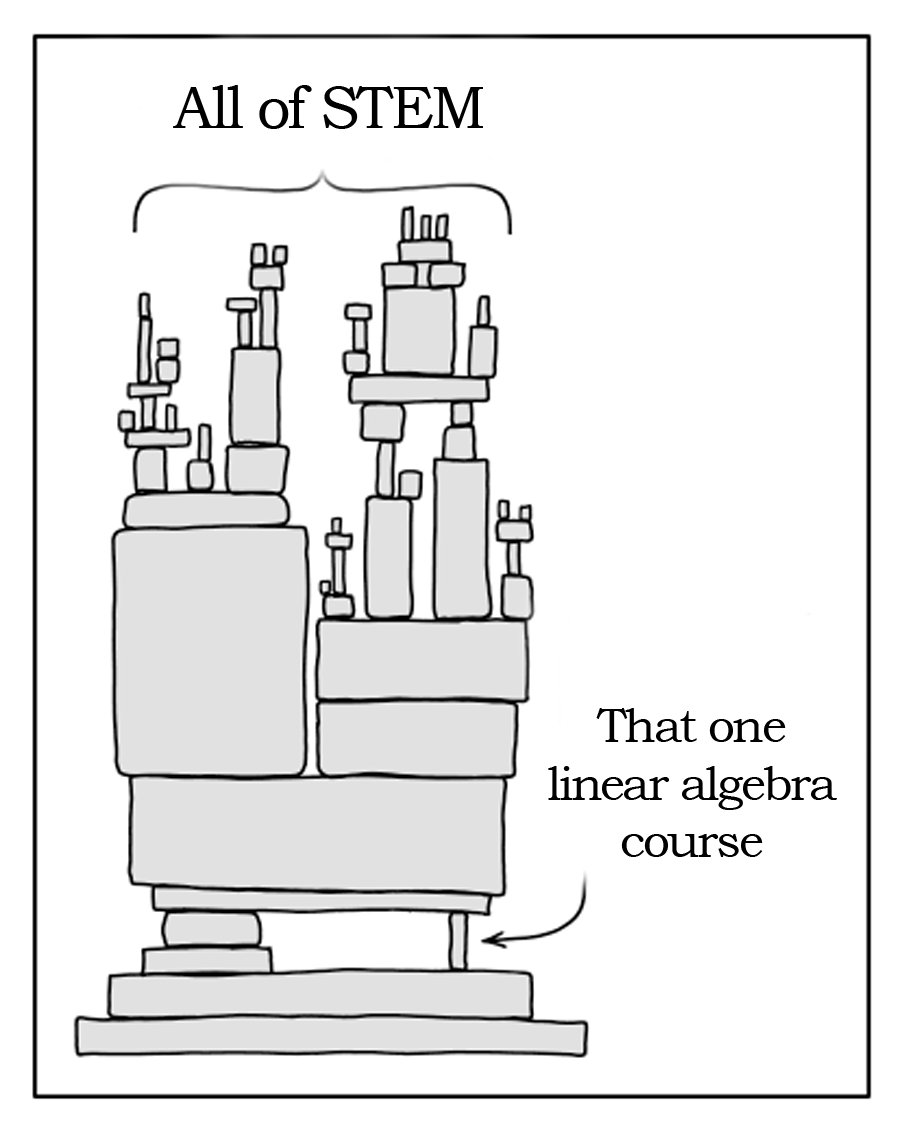
\includegraphics[scale=0.225]{stem_linal.png}
\end{column}	
\begin{column}[c]{0.25\textwidth}
\maroon{\large Coming up:\\~\\ Applications of Matrix Algebra}
\end{column}	
\end{columns}
\end{frame}

%%%%%%%%%%%%%%%%%%%%
\begin{frame}{Network Theory}
A network of connections can be expressed as an adjacency matrix.
$$ M=\left(\begin{array}{cccc}
m_{11} & m_{12} & \cdots & m_{1 n} \\
m_{21} & m_{22} & \cdots & m_{2 n} \\
\vdots & \vdots & \ddots & \vdots \\
m_{n 1} & m_{n 2} & \cdots & m_{n n}
\end{array}\right)  $$

where 
$$ m_{ij} = \begin{cases}
	1 \quad \text{if there is a direct link from $i$ to $j$} \\
	0 \quad \text{otherwise}
\end{cases} $$
\end{frame}

%%%%%%%%%%%%%%%%%%%%
\begin{frame}{Network Theory}
\vspace{-0.25cm}
Consider the following network: \vspace{-0.25cm}
\begin{center}
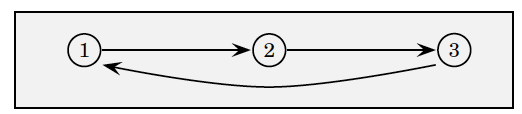
\includegraphics[scale=0.5]{eg.png}
$$ M=\left(\begin{array}{lll}
0 & 1 & 0 \\
0 & 0 & 1 \\
1 & 0 & 0
\end{array}\right), \quad M^2=\left(\begin{array}{lll}
0 & 0 & 1 \\
1 & 0 & 0 \\
0 & 1 & 0
\end{array}\right), \quad M^3=\left(\begin{array}{lll}
1 & 0 & 0 \\
0 & 1 & 0 \\
0 & 0 & 1
\end{array}\right) $$	
\end{center}
The matrices $M, M^2, M^3$ give the nodes reachable in one, two and three
steps from any initial node.
\end{frame}

%%%%%%%%%%%%%%%%%%%%
\begin{frame}{Network Theory}
\vspace{-0.25cm}
Consider the sum:
$$ S_k = M + M^2 + M^3 +...+M^k $$
The $(i, j)$ element of $S_k$ gives the number of paths of length $k$ or
less, from $i$ to $j$. \\~\\

For the previous example:
$$S_3 = M + M^2 + M^3 = \left(\begin{array}{lll}
1 & 1 & 1 \\
1 & 1 & 1 \\
1 & 1 & 1
\end{array}\right)$$
So there is one way to go from any node to any other in three or fewer steps.
\end{frame}

%%%%%%%%%%%%%%%%%%%%
\begin{frame}{Uses of Network Theory}
Network theory can be used to model \\
\begin{witemize}
  \item Interconnectedness of financial institutions (to predict risk of banking collapses)
  \item Interconnectedness of the countries in world trade
  \item Predicting supply chain risk
\end{witemize}
\end{frame}

%%%%%%%%%%%%%%%%%%%%
\begin{frame}{Markov Chain}
\begin{witemize}
    \item A Markov Chain can model the transition between different states.
    \item Example: Employment (E) and Unemployment (U).
 \item Transition matrix:
\[
P = \begin{pmatrix}
P(E \rightarrow E) & P(U \rightarrow E) \\
P(E \rightarrow U) & P(U \rightarrow U)
\end{pmatrix}
= \begin{pmatrix}
0.9 & 0.2 \\
0.1 & 0.8
\end{pmatrix}
\]
\item Say the initial state vector is:
$$ \pi(0) =  \begin{bmatrix}
\pi_E(0)  \\
\pi_U(0)
\end{bmatrix} =  \begin{bmatrix}
0.8  \\
0.2
\end{bmatrix}
 $$
 \end{witemize}
\end{frame}

\begin{frame}{Transition Matrix}
After one period, the state distribution is:
$$  \pi(1) = \begin{bmatrix}
\pi_E(1)  \\
\pi_U(1)
\end{bmatrix} = P \pi(0) = \begin{bmatrix}
0.9 & 0.2 \\
0.1 & 0.8
\end{bmatrix} \begin{bmatrix}
0.8  \\
0.2
\end{bmatrix}
 = \begin{bmatrix}
0.76  \\
0.24
\end{bmatrix}$$ \\
After $t$ periods:
$$ \pi(t) = P^t \pi(0) $$
\end{frame}

%%%%%%%%%%%%%%%% 
 \begin{frame}{Ordinary Least Squares}
 \vspace{-0.25cm}
Linear model with $k$ variables:
  $$ Y_i = \beta_0 + \beta_1 X_{i1} + \beta_2 X_{i2} + \hdots + \beta_k X_{ik} + \varepsilon_i $$
  where $i = 1,...,n$ denotes $n$ observations. \\
  Denote $$ Y  = \begin{bmatrix} Y_1 \\ Y_2 \\  \vdots \\ Y_n  \end{bmatrix}_{n \times 1},    
  \beta  = \begin{bmatrix} \beta_0 \\ \beta_1  \\ \vdots \\ \beta_k \end{bmatrix}_{k \times 1},  
  \boldsymbol{X} = \begin{bmatrix} 1 & X_{11} & \hdots & X_{1k} \\ 1 & X_{12} & \hdots & X_{2k}  \\ \vdots & \vdots \\ 1 & X_{1n} & \hdots & X_{nk}  \end{bmatrix}_{n \times k},  
  \varepsilon  = \begin{bmatrix} \varepsilon_1 \\ \varepsilon_2 \\ \vdots \\ \varepsilon_n  \end{bmatrix}_{n \times 1} $$
  Then, 
  $$ Y = X \beta + \varepsilon  \quad \quad \text{OLS estimator: } \hat{\beta} = (X'X)^{-1} X'Y$$
\end{frame}

%%%%%%%%%%%%%%%%%%%%
\begin{frame}{Natural Language Processing (NLP)}
\vspace{-0.75em}
\begin{witemize}
  \item Bag of Words (BoW) model is a simple and widely used method in NLP
  \item Transform text into fixed-length vectors by counting how many times each word appears in a document
  \item Example: 
  \begin{itemize}
  \item Doc1: ``the cat sat on the mat''
  \item Doc2: ``the dog sat on the log''
  \item Vocabulary for these documents: $[the, cat, sat, on, mat, dog, log]$
  \item Vector for Doc1: $[2, 1, 1, 1, 1, 0, 0]$
  \item Vector for Doc2: $[2, 0, 1, 1, 0, 1, 1]$
\end{itemize}
\item Calculate similarity between document vectors to classify documents into predefined classes
\end{witemize}
\end{frame}

 %%%%%%%%%%%%%%%% 
 \begin{frame}{What's next?}
 \begin{witemize}
  \item Quiz 2 next week will cover all of Linear Algebra
  \item Notes for reviewing Linear Algebra uploaded (not a substitute for the textbook for understanding concepts)
  \item We will move on to differential calculus next week
\end{witemize}
 \end{frame}
 
 %%%%%%%%%%%%%%%% 
 \begin{frame}{Homework Problems}
 Textbook reference: Sections 5.3-5.5 \\~\
 \begin{witemize}
\item Exercise 5.3: 1, 4, 5, 8
\item Exercise 5.4: 2, 3, 4, 6, 7
  \item Exercise 5.5: 1, 2, 3 (a) (d)
\end{witemize}

\end{frame}






\end{document}